\section{The Field of Play}\label{sec:field-of-play}

\subsection{Dimensions}
The field of play must be rectangular.
\added{Teams have the option of choosing to play on one of two sizes of fields: }
\begin{enumerate}
\item \textbf{\added{Single-size field}}, of size 6050\,mm$\times$ 4050\,mm
\item \textbf{\added{Double-size field}}, of size 8090\,mm$\times$ 6050\,mm
\end{enumerate}
The dimensions include boundary lines.
Dimensions of the field, goals, and special field areas are in millimetres and are shown in \autoref{fig:single_size_field}, \autoref{fig:double_size_field}.

\begin{figure}[ht] % ht = here / t = top / b = bottom
	\centering
	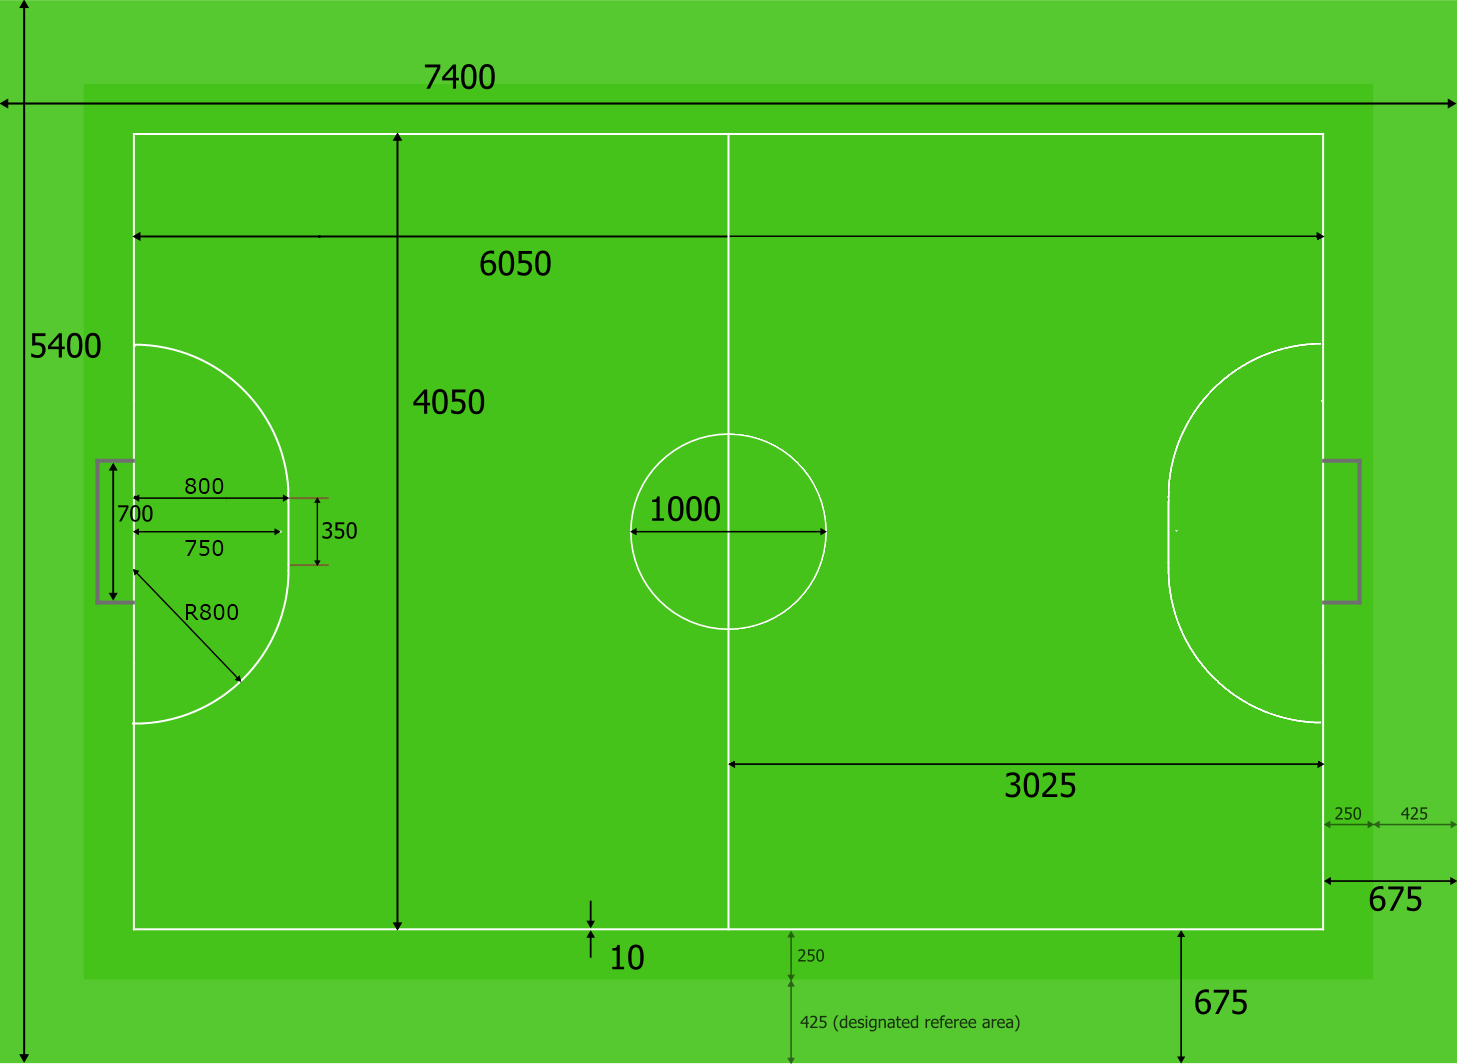
\includegraphics[width=0.8\columnwidth]{img/field_2012_drawing.png}
	\caption{The field dimensions of the single-size field}
	\label{fig:single_size_field}
\end{figure}

\begin{figure}[ht] % ht = here / t = top / b = bottom
	\centering
	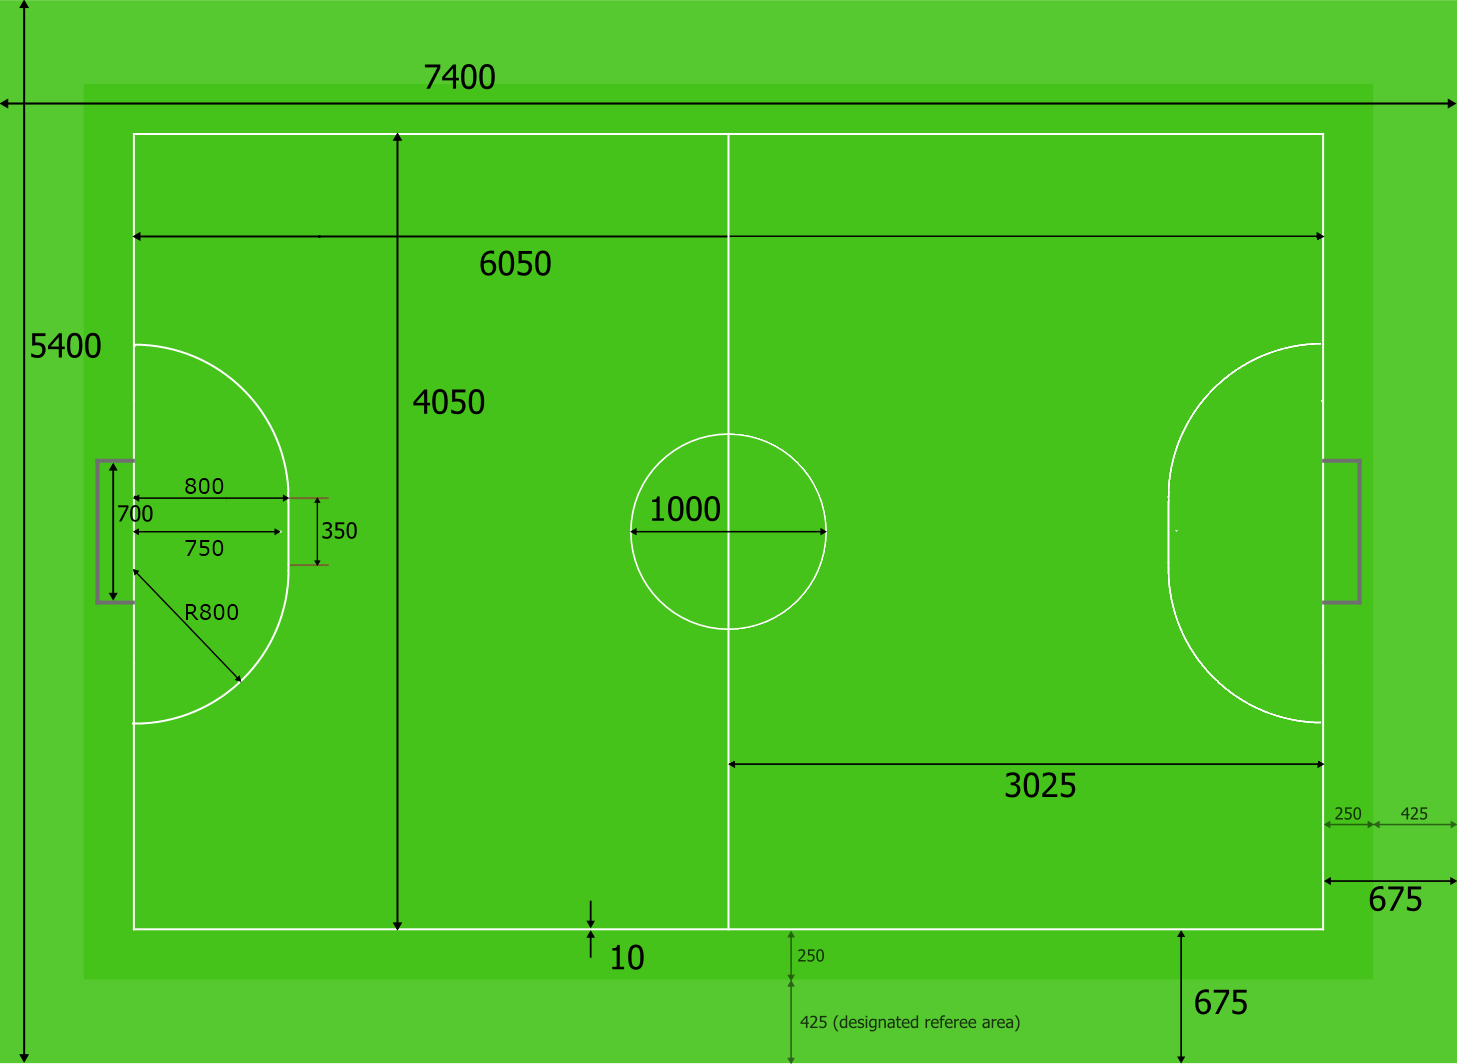
\includegraphics[width=0.8\columnwidth]{img/field_2012_drawing.png}
	\caption{The field dimensions of the double-size field}
	\label{fig:double_size_field}
\end{figure}

\added{
The rules in this rule book apply identically to both sizes of fields, unless otherwise explicitly mentioned.
Specifically, the following rules have differences in their application to the two field sizes:
}
\begin{enumerate}
\item \added{The number and length of timeouts in \autoref{subsec:duration-of-the-match-timeouts}}
\item \added{The robot speed limit during stoppage of play in \autoref{subsec:fouls-and-misconduct-disciplinary-sanctions}}
\end{enumerate}

\subsection{Field Surface}
The playing surface is green felt mat or carpet.
The floor under the carpet is level, flat, and hard.

The field surface will continue for 675\,mm beyond the boundary lines on all sides.
The outer 425\,mm of this runoff area are used as a designated referee walking area (see \autoref{sec:referee}).
At the edge of the field surface, a 100\,mm tall wall will prevent the ball and robots from running off the edge.

\subsection{Field Markings}
The field of play is marked with lines.
Lines belong to the areas of which they are boundaries.

The two longer sides are called touch boundaries.
The two shorter sides are called goal boundaries.

All lines are 10\,mm wide and painted white.

The field of play is divided into two halves by a halfway line.

The centre mark is indicated at the midpoint of the halfway line.
A circle with a diameter of 1000\,mm is marked around it.

\subsection{The Defence Area}
A defence area is defined at each end of the field as follows:

Two quarter circles with a radius of 800\,mm are drawn on the field of play.
These quarter circles are connected by a line parallel to the goal line.
The exact configuration is depicted in figure \ref{fig:sslfield}.

The area bounded by this arc and the goal line is the defence area.

\subsection{Penalty Mark}
Within each defence area a penalty mark is made 750\,mm from the midpoint between the goalposts and equidistant to them.
The mark is a 10\,mm diameter circle of white paint.

\subsection{Goals}
Goals must be placed on the centre of each goal boundary.

They consist of two 160\,mm vertical side walls joined at the back by a 160\,mm vertical rear wall.
The inner face of the goal has to be covered with an energy absorbing material such as foam to help absorb ball impacts and lessen the speed of deflections.
The goal walls, edges, and tops are white in color.

There is a round steel cross bar that runs across the top of the goalmouth and parallel to the goal line.
It is no larger than 10\,mm in diameter, but is sufficiently strong to deflect the ball.
The bottom of the bar is 155\,mm from the field surface, and the bar is dark in color to minimise interference with vision systems.
The top of the goal is covered in a thin net to prevent the ball from entering the goal from above.
It is attached securely to the cross bar and goal walls.

The distance between the side walls is 700\,mm.
The goal is 180\,mm deep.
The distance from the lower edge of the crosswire to the playing surface is 150\,mm.

The floor inside the goalmouth is the same as the rest of the playing surface.

The goal walls are 20\,mm thick.

Goals must be anchored securely to field surface.

\begin{figure}[ht] % ht = here / t = top / b = bottom
	\centering
	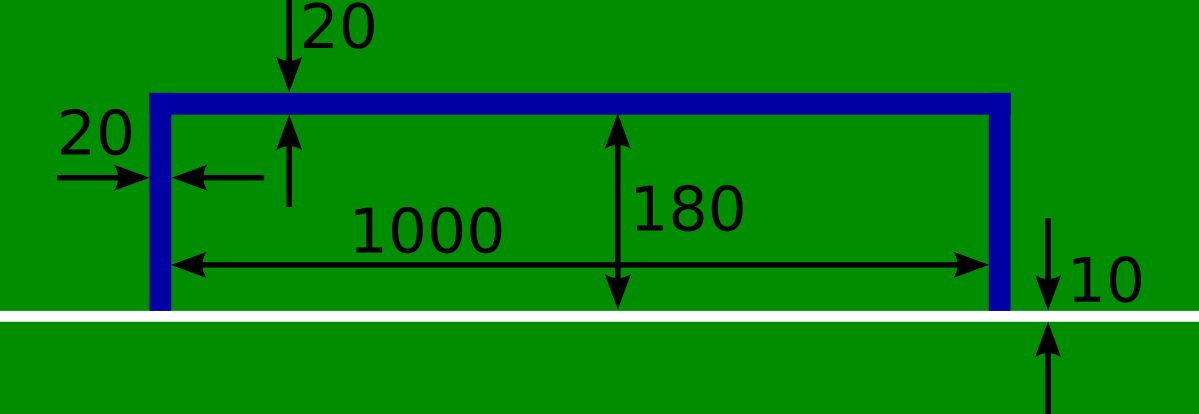
\includegraphics[width=0.5\columnwidth]{img/goal_detail.png}
	\caption{The Goal in detail}
	\label{fig:sslgoal}
\end{figure}

\subsection{Equipment Mounting Bar}
A mounting bar will be provided 4\,m above the field.
The bar will run above the midline of the field from goal to goal.
The bar should be mounted securely so that it does not swing or sway under a small external force, and it should not bend or twist significantly when the weight of typical video equipment is added.

\subsection{Shared Vision System}
Each field is provided with a shared central vision server and a set of shared cameras.
This shared vision equipment uses the community-maintained \textbf{SSL-Vision}\footnote{\url{http://codegooglecom/p/ssl-vision/}} software to provide localization data to teams via Ethernet in a packet format that is to be announced by the shared vision system developers before the competition.
Teams need to ensure that their systems are compatible with the shared vision system output and that their systems are able to handle the typical properties of real-world sensory data as provided by the shared vision system (including noise, latency, or occasional failed detections and misclassifications).

Besides the shared vision equipment, teams are \emph{not} allowed to mount their own cameras or other external sensors, unless specifically announced or permitted by the respective competition organisers.

The shared vision system in each field is maintained by one or more vision experts.
The procedure of selection of these experts will be announced by the competition organisers.
\autoref{app:vision-experts} describes the duties of the vision experts.

\subsection*{Decisions of the Small Size League Technical Committee}
\begin{enumerate}
\item
The local organising committee should aim to provide uniform, diffuse lighting conditions of approximately 500\,lux or brighter.
No special lighting equipment will necessarily be used to provide these conditions.
The brightness is not guaranteed nor expected to be fully uniform across the field surface.
Teams are thus expected to cope with the variations that will occur when using ambient lighting.
The organising committee will release details of the lighting arrangements to the competitors as early as practical.

\item
No kind of commercial advertising, whether real or virtual, is permitted on the field of play and field equipment (including the goal nets and the areas they enclose) from the time the teams enter the field of play until they have left it at half-time and from the time the teams re-enter the field of play until the end of the match.
In particular, no advertising material of any kind may be displayed inside the goals or walls.
No extraneous equipment (cameras, microphones, etc.) may be attached to these items.

\item
The specific color and texture of the surface is not specified and may vary from competition to competition (just as real soccer fields vary).
The surface underneath the carpet will be level and hard.
Examples of approved surfaces include: cement, linoleum, hardwood flooring, plywood, ping-pong tables and particle board; carpeted or cushioned surfaces are not allowed.
Every effort shall be made to ensure that the surface is flat; however, it is up to individual teams to design their robots to cope with slight curvatures of the surface.
\end{enumerate}